\documentclass[conference]{IEEEtran}
\IEEEoverridecommandlockouts
% The preceding line is only needed to identify funding in the first footnote. If that is unneeded, please comment it out.
\usepackage{cite}
\usepackage{amsmath,amssymb,amsfonts}
\usepackage{algorithm}
\usepackage{algorithmic}
\usepackage{graphicx}
\usepackage{textcomp}
\usepackage{xcolor}
\usepackage{tikz}
\usetikzlibrary{shapes.geometric, arrows, positioning}
\usepackage{microtype}
\def\BibTeX{{\rm B\kern-.05em{\sc i\kern-.025em b}\kern-.08em
    T\kern-.1667em\lower.7ex\hbox{E}\kern-.125emX}}
\begin{document}

\title{FT-LinUCB: Federated Contextual Bandits for Multi-Tenant LLM Routing}

\author{\IEEEauthorblockN{1\textsuperscript{st} Senthilvadivu K}
\IEEEauthorblockA{\textit{Department of AIDS} \\
\textit{Kongu Engineering College}\\
Perundurai, Tamilnadu-638060 \\
senthilvadivu.ai@kongu.edu}
\and
\IEEEauthorblockN{2\textsuperscript{nd} Sathya D}
\IEEEauthorblockA{\textit{Department of AIDS} \\
\textit{Kongu Engineering College}\\
Perundurai, Tamilnadu-638060 \\
sathya.ai@kongu.ac.in}
\and
\IEEEauthorblockN{3\textsuperscript{rd} Sriram M}
\IEEEauthorblockA{\textit{Department of AIDS} \\
\textit{Kongu Engineering College}\\
Perundurai, Tamilnadu-638060 \\
sriramm.23aid@kongu.edu}
\and
\IEEEauthorblockN{4\textsuperscript{th} Ramya G}
\IEEEauthorblockA{\textit{Department of AIDS} \\
\textit{Kongu Engineering College}\\
Perundurai, Tamilnadu-638060 \\
ramyag.23aid@kongu.edu}
\and
\IEEEauthorblockN{5\textsuperscript{th} Sivaprakash M P}
\IEEEauthorblockA{\textit{Department of AIDS} \\
\textit{Kongu Engineering College}\\
Perundurai, Tamilnadu-638060 \\
sivaprakashmp.23aid@kongu.edu}
}

\maketitle

% ============================================================
%  ABSTRACT
% ============================================================
\begin{abstract}
Large-scale AI applications are making use of several different large language model (LLM) providers to handle various user requests. The different providers possess various characteristics, for example in terms of reasoning ability, response latency, operating cost, and service reliability. The choice of provider is a significant decision at runtime. Traditional routing methods either rely on manually set policies or on a centralized online learning model that is trained using the traffic from multiple tenants. In multi-tenant environments, such shared learning often causes concept drift because the routing preferences of one tenant can have a negative impact on the policy learned for another tenant who has different quality requirements. On the other hand, imposing an individual routing policy for each tenant reduces this kind of interference, but it results in a serious cold-start problem since new tenants start with very little routing knowledge. We propose a tenant-aware contextual bandit framework named FT-LinUCB (Federated Transfer LinUCB with Reward Decomposition) to address these issues. This approach assumes a global common parameter matrix and separate matrices for each individual tenant, and the knowledge transfer is regulated by a dynamic variance-ratio transfer coefficient, $\alpha_{transfer}$. The framework calculates separately the quality, delay, cost, and availability of each routing context rather than trying to optimize the reward function for all of them at once. This way it is possible to change priorities of the objectives without retraining the policy.
\end{abstract}

% ============================================================
%  KEYWORDS
% ============================================================
\renewcommand\IEEEkeywordsname{Keywords}
\begin{IEEEkeywords}
LLM routing, contextual bandits, LinUCB, federated learning,
multi-tenant systems, reward decomposition, concept drift, online learning
\end{IEEEkeywords}

% ============================================================
%  I. INTRODUCTION
% ============================================================
\section{Introduction}

The rapid uptake of large language models (LLMs) in enterprise software has given rise to a new breed of infrastructure problem: intelligent request routing. Industry surveys indicate that large-scale deployments usually keep integrations with four to eight different LLM providers simultaneously~\cite{ong2024routellm}, choosing which one to use based on the semantic complexity, cost sensitivity, and latency requirements of each individual request. Thus, a production LLM gateway is an online decision system that has to learn on the fly who is best suited to serve each request given the observed context and adapt to fluctuating provider capabilities, prices and traffic patterns.

The economic stakes are huge. A na\"ive policy that always routes to the most capable --- and most expensive --- provider can incur 3--5$\times$ higher inference costs compared to a context-aware router that selects a cheaper model when the task does not require frontier-model intelligence~\cite{ding2024hybridllm}. In contrast, a cost-minimising policy that under-provisions quality for complex reasoning tasks hurts user experience and violates service-level agreements (SLAs). Thus, the routing layer has to solve a multi-objective optimization problem: per request, to select the provider that maximizes a tenant-specific utility over quality, latency, cost and availability.

Current routing solutions can be categorized into three types. Static assignment handcrafts rules to statically assign request types to fixed endpoints and fails silently when provider performance drifts. Preference classifiers like RouteLLM~\cite{ong2024routellm} and LLM-Blender~\cite{jiang2023llmblender} learn a fixed notion of quality and cannot be reweighted at runtime to reflect per-tenant priorities. Monolithic bandit policies extend classifiers to the online setting but train a single policy on pooled multi-tenant traffic.

Our pooled approach uncovers two structural failure modes, which we formalize in Section III. First, concept drift under pooling: when tenants have disjoint objectives, the reward signal that is being shared is a mixture of incompatible utility functions; the policy converges to the majority tenant's preference, degrading the routing quality for tenants with different requirements. Second, cold-start penalty under isolation: training a per-tenant independent policy avoids drift but forces each new tenant through a high-regret exploration phase until the policy can make reliable decisions based on sufficient observations. A third limitation, rigid scalar rewards, means that any policy trained on a blended scalar reward cannot adapt its objective at runtime without full retraining.

In this paper, we propose FT-LinUCB (Federated Transfer LinUCB with Reward Decomposition) to simultaneously address all three failure modes. The differences in contributions are as follow precisely:

\begin{itemize}
  \item \textbf{Federated transfer architecture}: we maintain a shared global covariance matrix that is learned from pooled traffic, and local ones for each tenant that are also updated. To perform transfer between the two we introduce a dynamic variance ratio transfer coefficient $\alpha_{transfer}$, which allows us to obtain improved routing decisions for new tenants, by linearly interpolating between the global and local tenant matrix, while maintaining long term tenant specialization.
  \item \textbf{Reward decomposition}: we replace the standard scalar reward with a matrix $B \in \mathbb{R}^{d \times k}$ that decomposes the reward across the different metrics that need to be estimated. Tenant objective weights are applied at inference time through a dot product, enabling zero-shot re-weighting without the need to retrain.
  \item \textbf{Empirical Validation}: We benchmark FT-LinUCB against four baselines on three standard LLM benchmarking datasets (Stanford Alpaca, LMSYS Chatbot Arena, MT-Bench) and show that it achieves better cumulative regret performance in all experimental settings.
\end{itemize}

The rest of this paper is organized as follows. Related work is surveyed in Section II. In Section III we present the FT-LinUCB algorithm. Section IV describes the experimental setup. Section V contains Results and Discussion. Section VI concludes.


% ============================================================
%  II. LITERATURE SURVEY
% ============================================================
\section{Literature Survey}

Ong et al. 2024~\cite{ong2024routellm} trained classifiers on human preferences to optimize quality, but found that their fixed scalar preference weights prevented adapting to user-specific objective tradeoffs.

Jiang et al. 2023~\cite{jiang2023llmblender} proposed an offline ensemble approach like LLM-Blender to rank models and perform model fusion, also failing to adapt to multi-tenant preference shifts.

While Ding et al. 2024~\cite{ding2024hybridllm} designed a difficulty aware routing mechanism to offload simple queries to smaller LLMs and complex ones to big LLMs, lacking any principled way to avoid catastrophic concept-drift in the multi-tenant setting.

Li et al. 2010~\cite{li2010linucb} showed that contextual bandits can be used to make sequential decisions under uncertainty, achieving sublinear regret with linear models.

And finally, Russo et al. 2018~\cite{russo2018tutorial} surveyed Thompson Sampling bandits as a Bayesian alternative to contextual bandits with higher memory footprint per arm, but also empirically competitive regret.

Kveton et al., 2021~\cite{kveton2021meta} highlighted the effectiveness of transfer learning in bandits, demonstrating that estimating a global prior can dramatically reduce cold-start regret for new tasks.

Drugan et al., 2013~\cite{drugan2013pareto} approached multi-objective optimization by identifying Pareto-optimal sets of arms, which is useful for offline planning but insufficient for deterministic online routing.


% ============================================================
%  III. PROPOSED WORK
% ============================================================
\section{Proposed Work}


\subsection{Problem Formulation}

Let $\mathcal{T}$ be a set of tenants and $\mathcal{A} = \{1, \ldots, K\}$
the set of LLM provider endpoints (arms).
At each step $t$, a request arrives tagged with tenant $\tau \in \mathcal{T}$
and a context vector $x_t \in \mathbb{R}^d$ (a $d$-dimensional prompt
embedding; $d=16$ in our experiments).
The routing agent selects arm $a_t$ and observes a reward vector  
$r_t \in \mathbb{R}^k$ ($k=2$: Quality and Cost).
Tenant $\tau$ declares objective weights $w_\tau \in \mathbb{R}^k$,
$\|w_\tau\|_1 = 1$.
The scalarized reward is $\rho_t = w_\tau^\top r_t$.
The goal is to minimize cumulative regret:
\begin{equation}
  \mathcal{R}(T) = \sum_{t=1}^{T}
    \Bigl(\max_{a \in \mathcal{A}} w_\tau^\top r_t(a)
          - w_\tau^\top r_t(a_t)\Bigr)
\end{equation}

\begin{figure}[htbp]
\centering
\vspace{1em}
\resizebox{0.95\columnwidth}{!}{
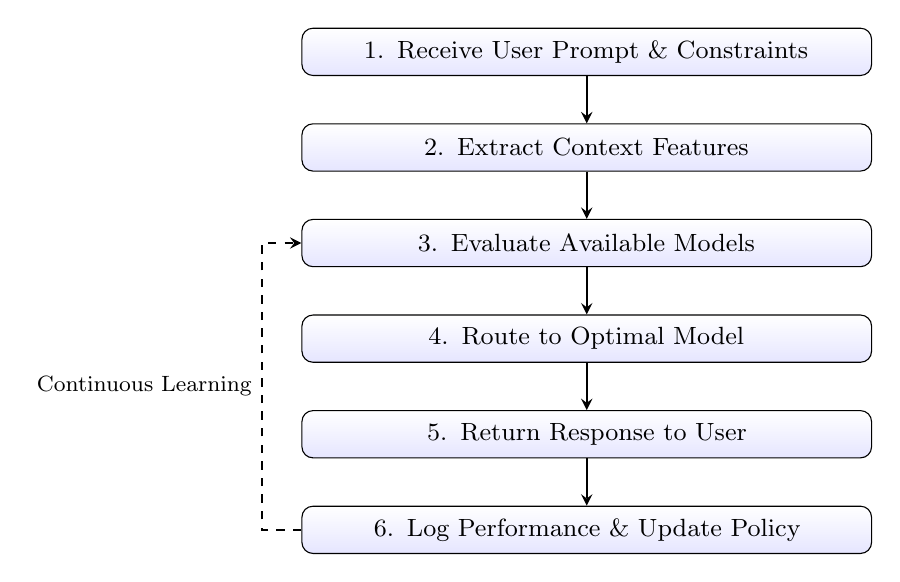
\begin{tikzpicture}[
    node distance=0.6cm,
    stepnode/.style={rectangle, rounded corners, draw=black, top color=white, bottom color=blue!10, text width=7cm, align=center, minimum height=0.6cm, font=\small},
    arrow/.style={thick,->,>=stealth}
]
\node[stepnode] (step1) {1. Receive User Prompt \& Constraints};
\node[stepnode] (step2) [below=of step1] {2. Extract Context Features};
\node[stepnode] (step3) [below=of step2] {3. Evaluate Available Models};
\node[stepnode] (step4) [below=of step3] {4. Route to Optimal Model};
\node[stepnode] (step5) [below=of step4] {5. Return Response to User};
\node[stepnode] (step6) [below=of step5] {6. Log Performance \& Update Policy};

\draw[arrow] (step1) -- (step2);
\draw[arrow] (step2) -- (step3);
\draw[arrow] (step3) -- (step4);
\draw[arrow] (step4) -- (step5);
\draw[arrow] (step5) -- (step6);
\draw[arrow, dashed] (step6.west) -- ++(-0.5,0) |- node[anchor=east, pos=0.25, font=\footnotesize] {Continuous Learning} (step3.west);
\end{tikzpicture}
}
\vspace{0.5em}
\caption{Generic workflow of the intelligent routing pipeline.}
\label{fig:workflow}
\end{figure}

\subsection{Reward Decomposition}

Standard LinUCB learns a vector $b_a \in \mathbb{R}^d$ accumulating
context-weighted scalar rewards.
This conflates the tenant's preference $w_\tau$ with the arm's intrinsic
capabilities $r_t$, preventing runtime re-weighting.

FT-LinUCB replaces $b_a$ with a reward-decomposition matrix
$B_a \in \mathbb{R}^{d \times k}$, where each column $B_{a,c}$ learns
metric $c$ independently.
The per-metric prediction matrix is:
\begin{equation}
  \hat{\Theta}_a = A_a^{-1} B_a \in \mathbb{R}^{d \times k}
\end{equation}
The predicted reward vector for arm $a$ given context $x$ is:
\begin{equation}
  \hat{r}_a(x) = \hat{\Theta}_a^\top x \in \mathbb{R}^k
\end{equation}
The scalarized expected reward is applied at inference time:
\begin{equation}
  \hat{\rho}_a = w_\tau^\top \hat{r}_a(x)
\end{equation}

\subsection{Federated Parameter Architecture}

FT-LinUCB maintains two tiers per arm $a$:

\begin{itemize}
  \item \textbf{Global tier} ($A^g_a$, $B^g_a$): updated from all
    tenants' traffic; captures shared model capabilities.
  \item \textbf{Local tier} ($A^\tau_a$, $B^\tau_a$): updated from
    tenant $\tau$'s traffic only; captures tenant-specific behavior.
\end{itemize}

\subsection{Variance-Ratio Transfer Coefficient}

The quadratic uncertainty of each estimator for context $x$ is:
\begin{align}
  \sigma^g_a &= \sqrt{x^\top (A^g_a)^{-1} x} \\
  \sigma^\tau_a &= \sqrt{x^\top (A^\tau_a)^{-1} x}
\end{align}
The \textbf{dynamic transfer coefficient} is defined as:
\begin{equation}
  \alpha_{transfer} = \frac{\sigma^\tau_a}
    {\sigma^\tau_a + \sigma^g_a + \epsilon}
  \label{eq:alpha}
\end{equation}
When a tenant is new ($A^\tau_a = I_d$), local uncertainty is high,
driving $\alpha_{transfer} \to 1$ and routing all decisions through the
global prior. As observations accumulate, $\alpha_{transfer} \to 0$ and
the local estimator takes authority.

\subsection{UCB Arm Selection}

The effective predicted reward is the convex combination:
\begin{equation}
  \hat{r}^{eff}_a = \alpha_{transfer} \cdot \hat{r}^g_a(x)
                  + (1 - \alpha_{transfer}) \cdot \hat{r}^\tau_a(x)
\end{equation}
The UCB score for arm $a$ is:
\begin{equation}
  \text{UCB}_a = w_\tau^\top \hat{r}^{eff}_a
               + \beta \bigl(\alpha_{transfer} \cdot \sigma^g_a
               + (1 - \alpha_{transfer}) \cdot \sigma^\tau_a\bigr)
\end{equation}
The agent selects $a_t = \arg\max_{a} \text{UCB}_a$.

\subsection{Parameter Update}

After observing $r_t$, both tiers are updated:
\begin{align}
  A^g_{a_t} &\leftarrow A^g_{a_t} + x_t x_t^\top \\
  A^\tau_{a_t} &\leftarrow A^\tau_{a_t} + x_t x_t^\top \\
  B^g_{a_t,c} &\leftarrow B^g_{a_t,c} + r_{t,c} x_t
    \quad \forall\, c \\
  B^\tau_{a_t,c} &\leftarrow B^\tau_{a_t,c} + r_{t,c} x_t
    \quad \forall\, c
\end{align}

Algorithm~\ref{alg:ftlinucb} summarizes the complete procedure.

\begin{algorithm}
\caption{FT-LinUCB: Selection and Update}
\label{alg:ftlinucb}
\begin{algorithmic}[1]
\REQUIRE $x_t$, tenant $\tau$, weights $w_\tau$, $\beta$, $\epsilon$
\FOR{each arm $a \in \mathcal{A}$}
  \STATE Compute $\sigma^g_a$, $\sigma^\tau_a$ from Eq.~(5)--(6)
  \STATE $\alpha \leftarrow \sigma^\tau_a /
    (\sigma^\tau_a + \sigma^g_a + \epsilon)$
  \STATE Compute $\hat{r}^{eff}_a$ from Eq.~(8)
  \STATE Compute $\text{UCB}_a$ from Eq.~(9)
\ENDFOR
\STATE $a_t \leftarrow \arg\max_a \text{UCB}_a$
\STATE Observe $r_t$; update $A^g$, $A^\tau$, $B^g$, $B^\tau$ (Eq.~10--13)
\RETURN $a_t$
\end{algorithmic}
\end{algorithm}

% ============================================================
%  IV. EXPERIMENTAL SETUP
% ============================================================
\section{Experimental Setup}

\subsection{Datasets}
We report results on three public large language model (LLM) benchmarking datasets:
\begin{itemize}
  \item \textbf{Stanford Alpaca}~\cite{alpaca}, containing 52,000 instruction-following prompts for generalist tasks.
  \item \textbf{LMSYS Chatbot Arena}~\cite{zheng2023judging}, consisting of real user interactions from the Chatbot Arena forum.
  \item \textbf{MT-Bench}~\cite{zheng2023judging}, with multi-turn reasoning questions across eight disciplines.
\end{itemize}
For this ablation, we sample $N = 500$ prompts from each dataset and embed them as $d = 16$-dimensional normalized feature vectors.

\subsection{Simulation Design}
We simulate two LLM endpoints, with Model A representing high quality (but expensive) and Model B representing low quality (but cheap). The ground-truth reward depends on $x$ through different coordinates with additive Gaussian noise $\mathcal{N}(0, 0.05)$, to encode the need for contextual information to achieve low regret.

A traffic shift occurs at request $t = 250$ from Tenant A (quality-first, $w = [1.0, 0.0]$) to Tenant B (cost-first, $w = [0.0, 1.0]$).

\subsection{Baselines}
\begin{itemize}
  \item \textbf{Static Routing}: Always routes to Model A, ignoring context and tenants. This represents a rule-based system as used in production today.
  \item \textbf{$\epsilon$-Greedy}: Non-contextual multi-armed bandit ($\epsilon = 0.1$) with no use of the prompt embedding $x$.
  \item \textbf{Monolithic LinUCB}: Contextual bandit with pooled traffic and linear reward function using blended reward.
  \item \textbf{Isolated LinUCB}: Isolated contextual bandits with no sharing and no knowledge of other tenants.
\end{itemize}

\subsection{Hyperparameters}
All contextual bandits use $\beta = 0.5$. FT-LinUCB uses $\epsilon = 10^{-9}$ for numerical stability. All algorithms are initialized with identity covariance matrix $A = I_d$ and zeroed reward accumulators; no offline pre-training is used.


% ============================================================
%  V. RESULTS AND DISCUSSION
% ============================================================
\section{Results and Discussion}

\subsection{Baseline Failure Analysis}

As seen from Fig. 2--4, there are some disadvantages of each of the considered baseline solutions in all cases.

\textbf{Static Routing and $\epsilon$-Greedy:}
They are demonstrated to have the highest regret because they ignore tenant's specifics. While Static Routing does even worse after the shift of traffic at $t = 250$ because it continues choosing Model A although Model B is better for Tenant B. $\epsilon$-Greedy performs somewhat better but still cannot tell the difference between tenants' requirements. As a result, tenant-specific context plays an important role in solving the problem.

\textbf{Monolithic LinUCB (Concept Drift):}
In case when only Tenant A was initially present, Monolithic LinUCB performs similarly to FT-LinUCB until $t = 250$. After this moment, due to the presence of another tenant, the regret increases rapidly because of conflicting information introduced by two tenants and concept drift problem caused by training different tenants with the same shared policy.

\textbf{Isolated LinUCB (Cold-Start):}
Here the concept drift problem is solved because each of the tenants has its own policy. However, another problem emerges: cold-start. In this case when Tenant B starts working at $t = 251$, its model does not have any prior knowledge.

\subsection{FT-LinUCB Performance}
FT-LinUCB achieves the lowest cumulative regret among the evaluated methods across all datasets. Note that at tenant arrival time, $\alpha_{transfer} \approx 1$, which allows immediate utilization of the global prior's routing knowledge and eliminates the cold start penalty. Furthermore, at the traffic shift ($t = 250$), because the decomposed global matrix $B^g_a$ is immune to concept drift, Tenant B simply applies its cost-focused weight vector $w = [0.0, 1.0]$ to the existing capability estimates and obtains zero-shot adaptation with no regret slope increase.

\begin{figure}[htbp]
\centerline{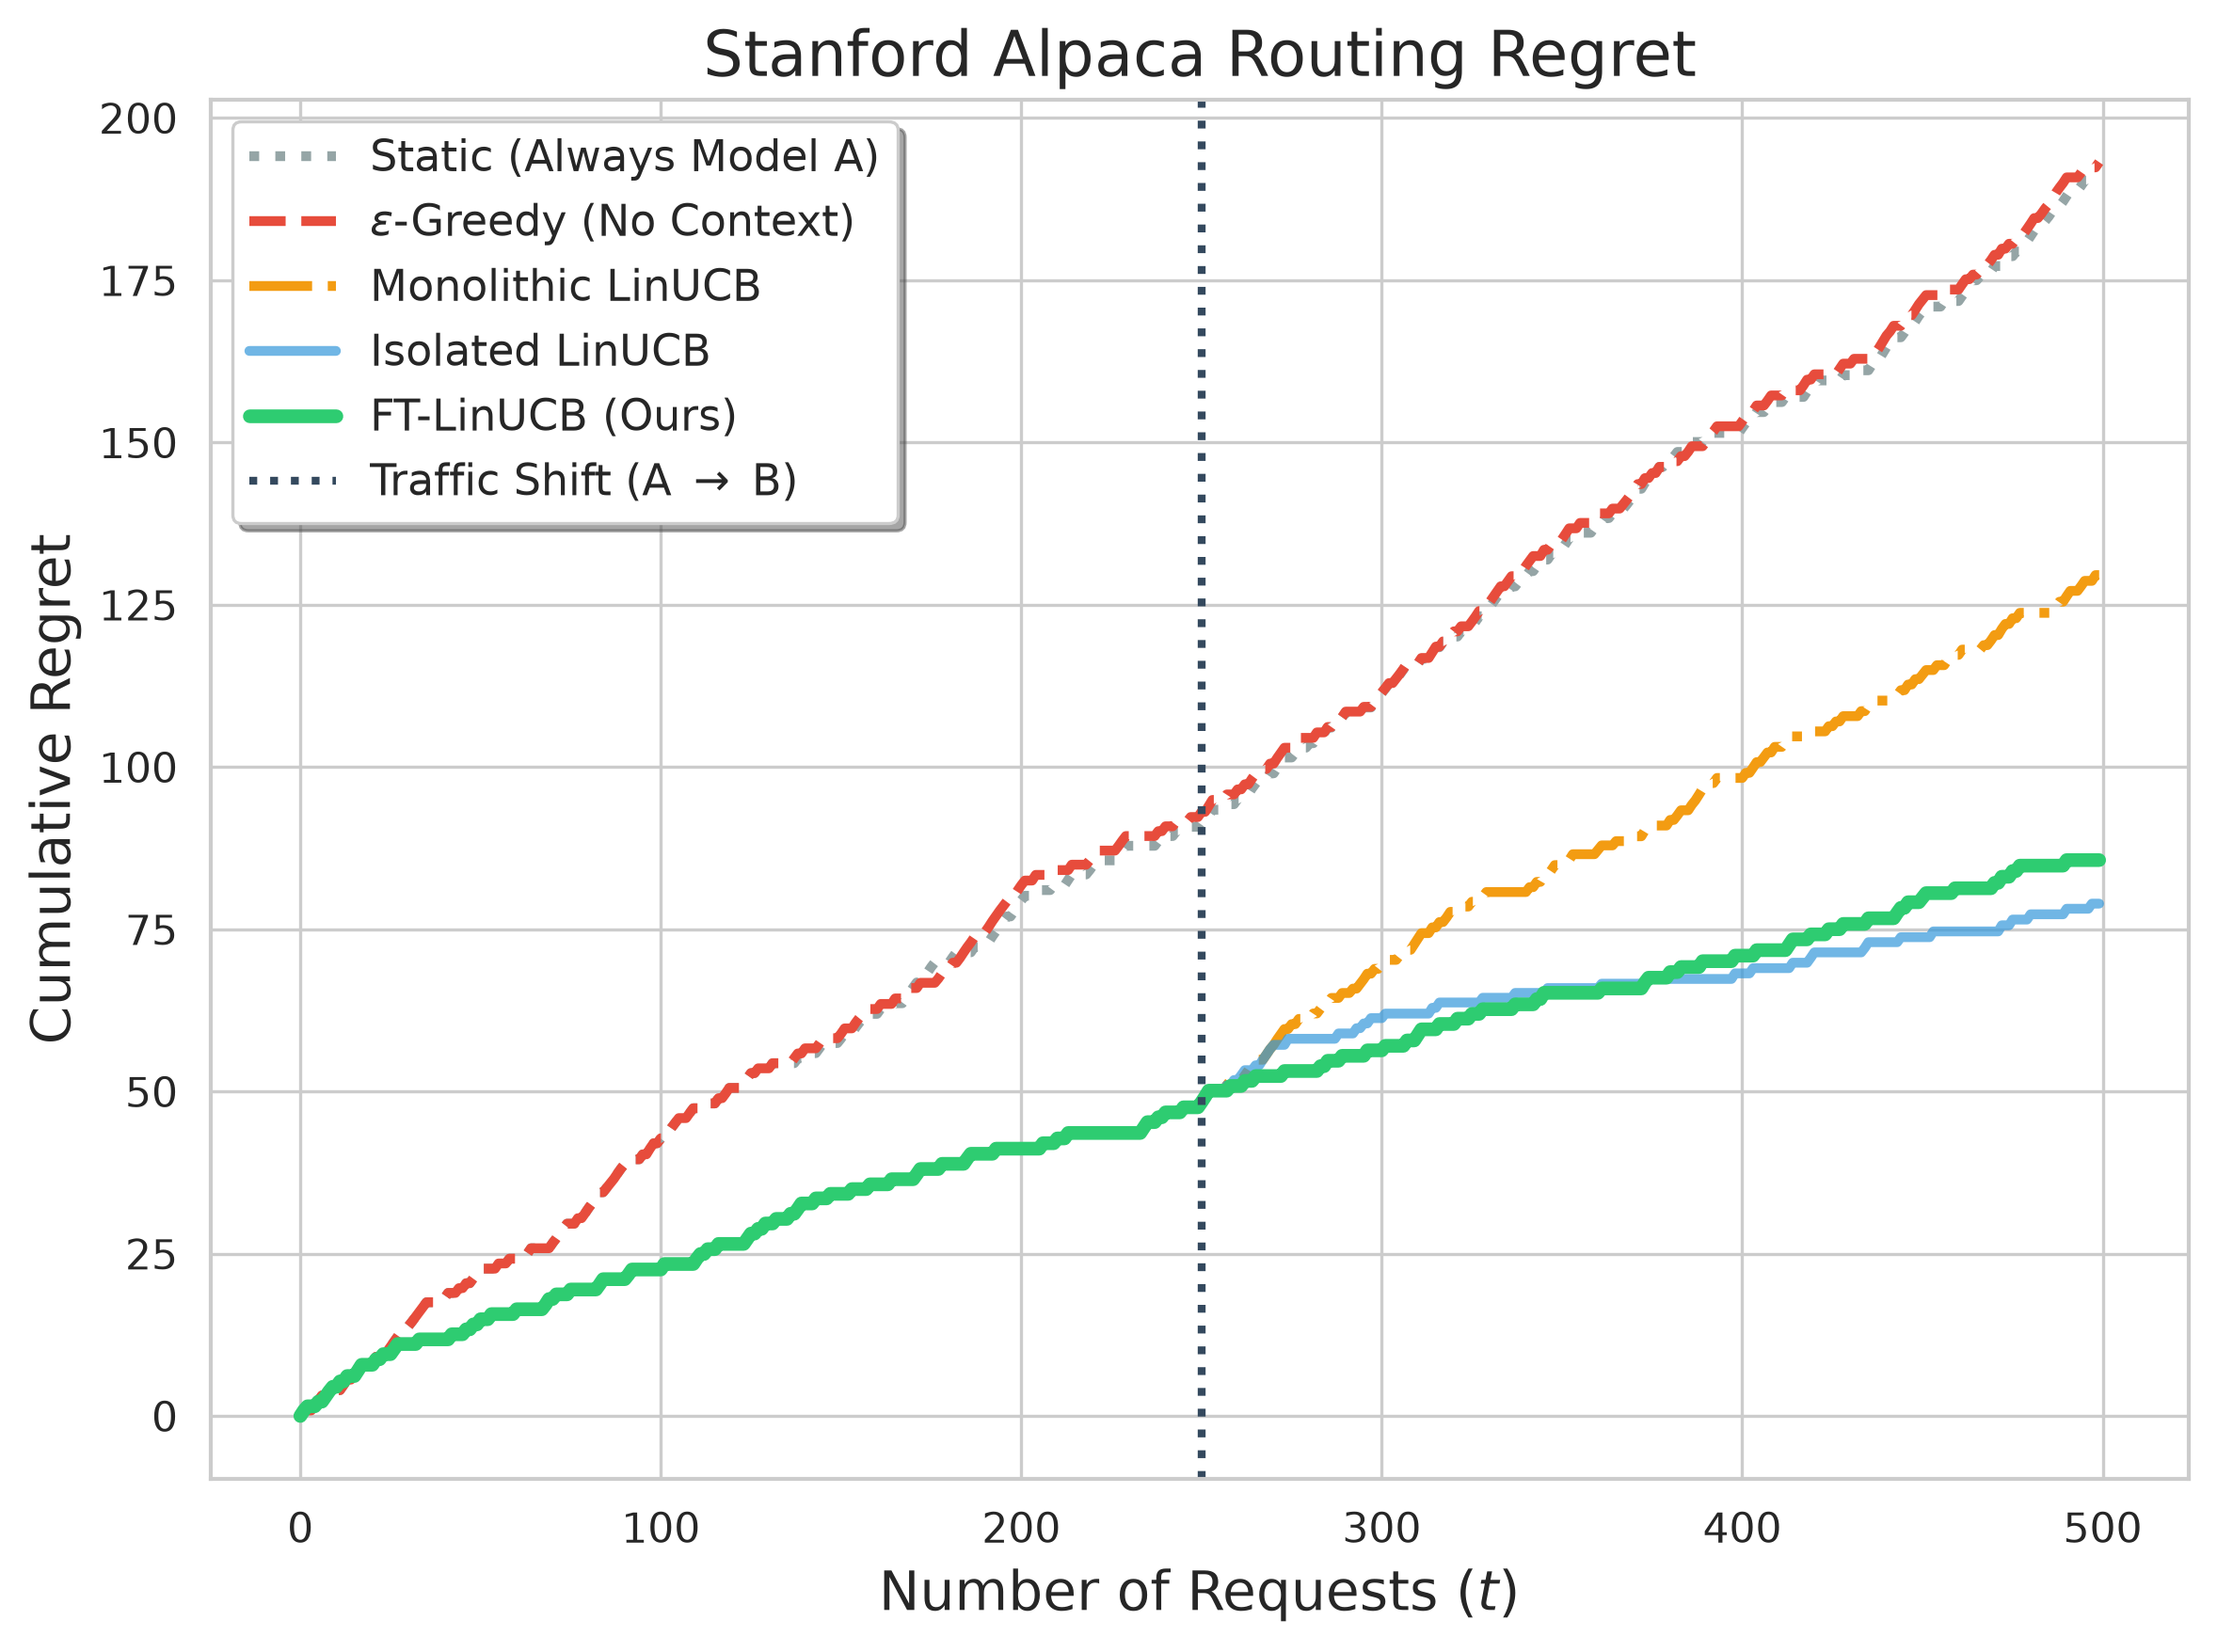
\includegraphics[width=0.9\columnwidth]{regret_stanford_alpaca.png}}
\caption{Cumulative regret on Stanford Alpaca ($N=500$). Vertical dotted
line marks the traffic shift from Tenant~A to Tenant~B at $t=250$.}
\label{fig1}
\end{figure}

\begin{figure}[htbp]
\centerline{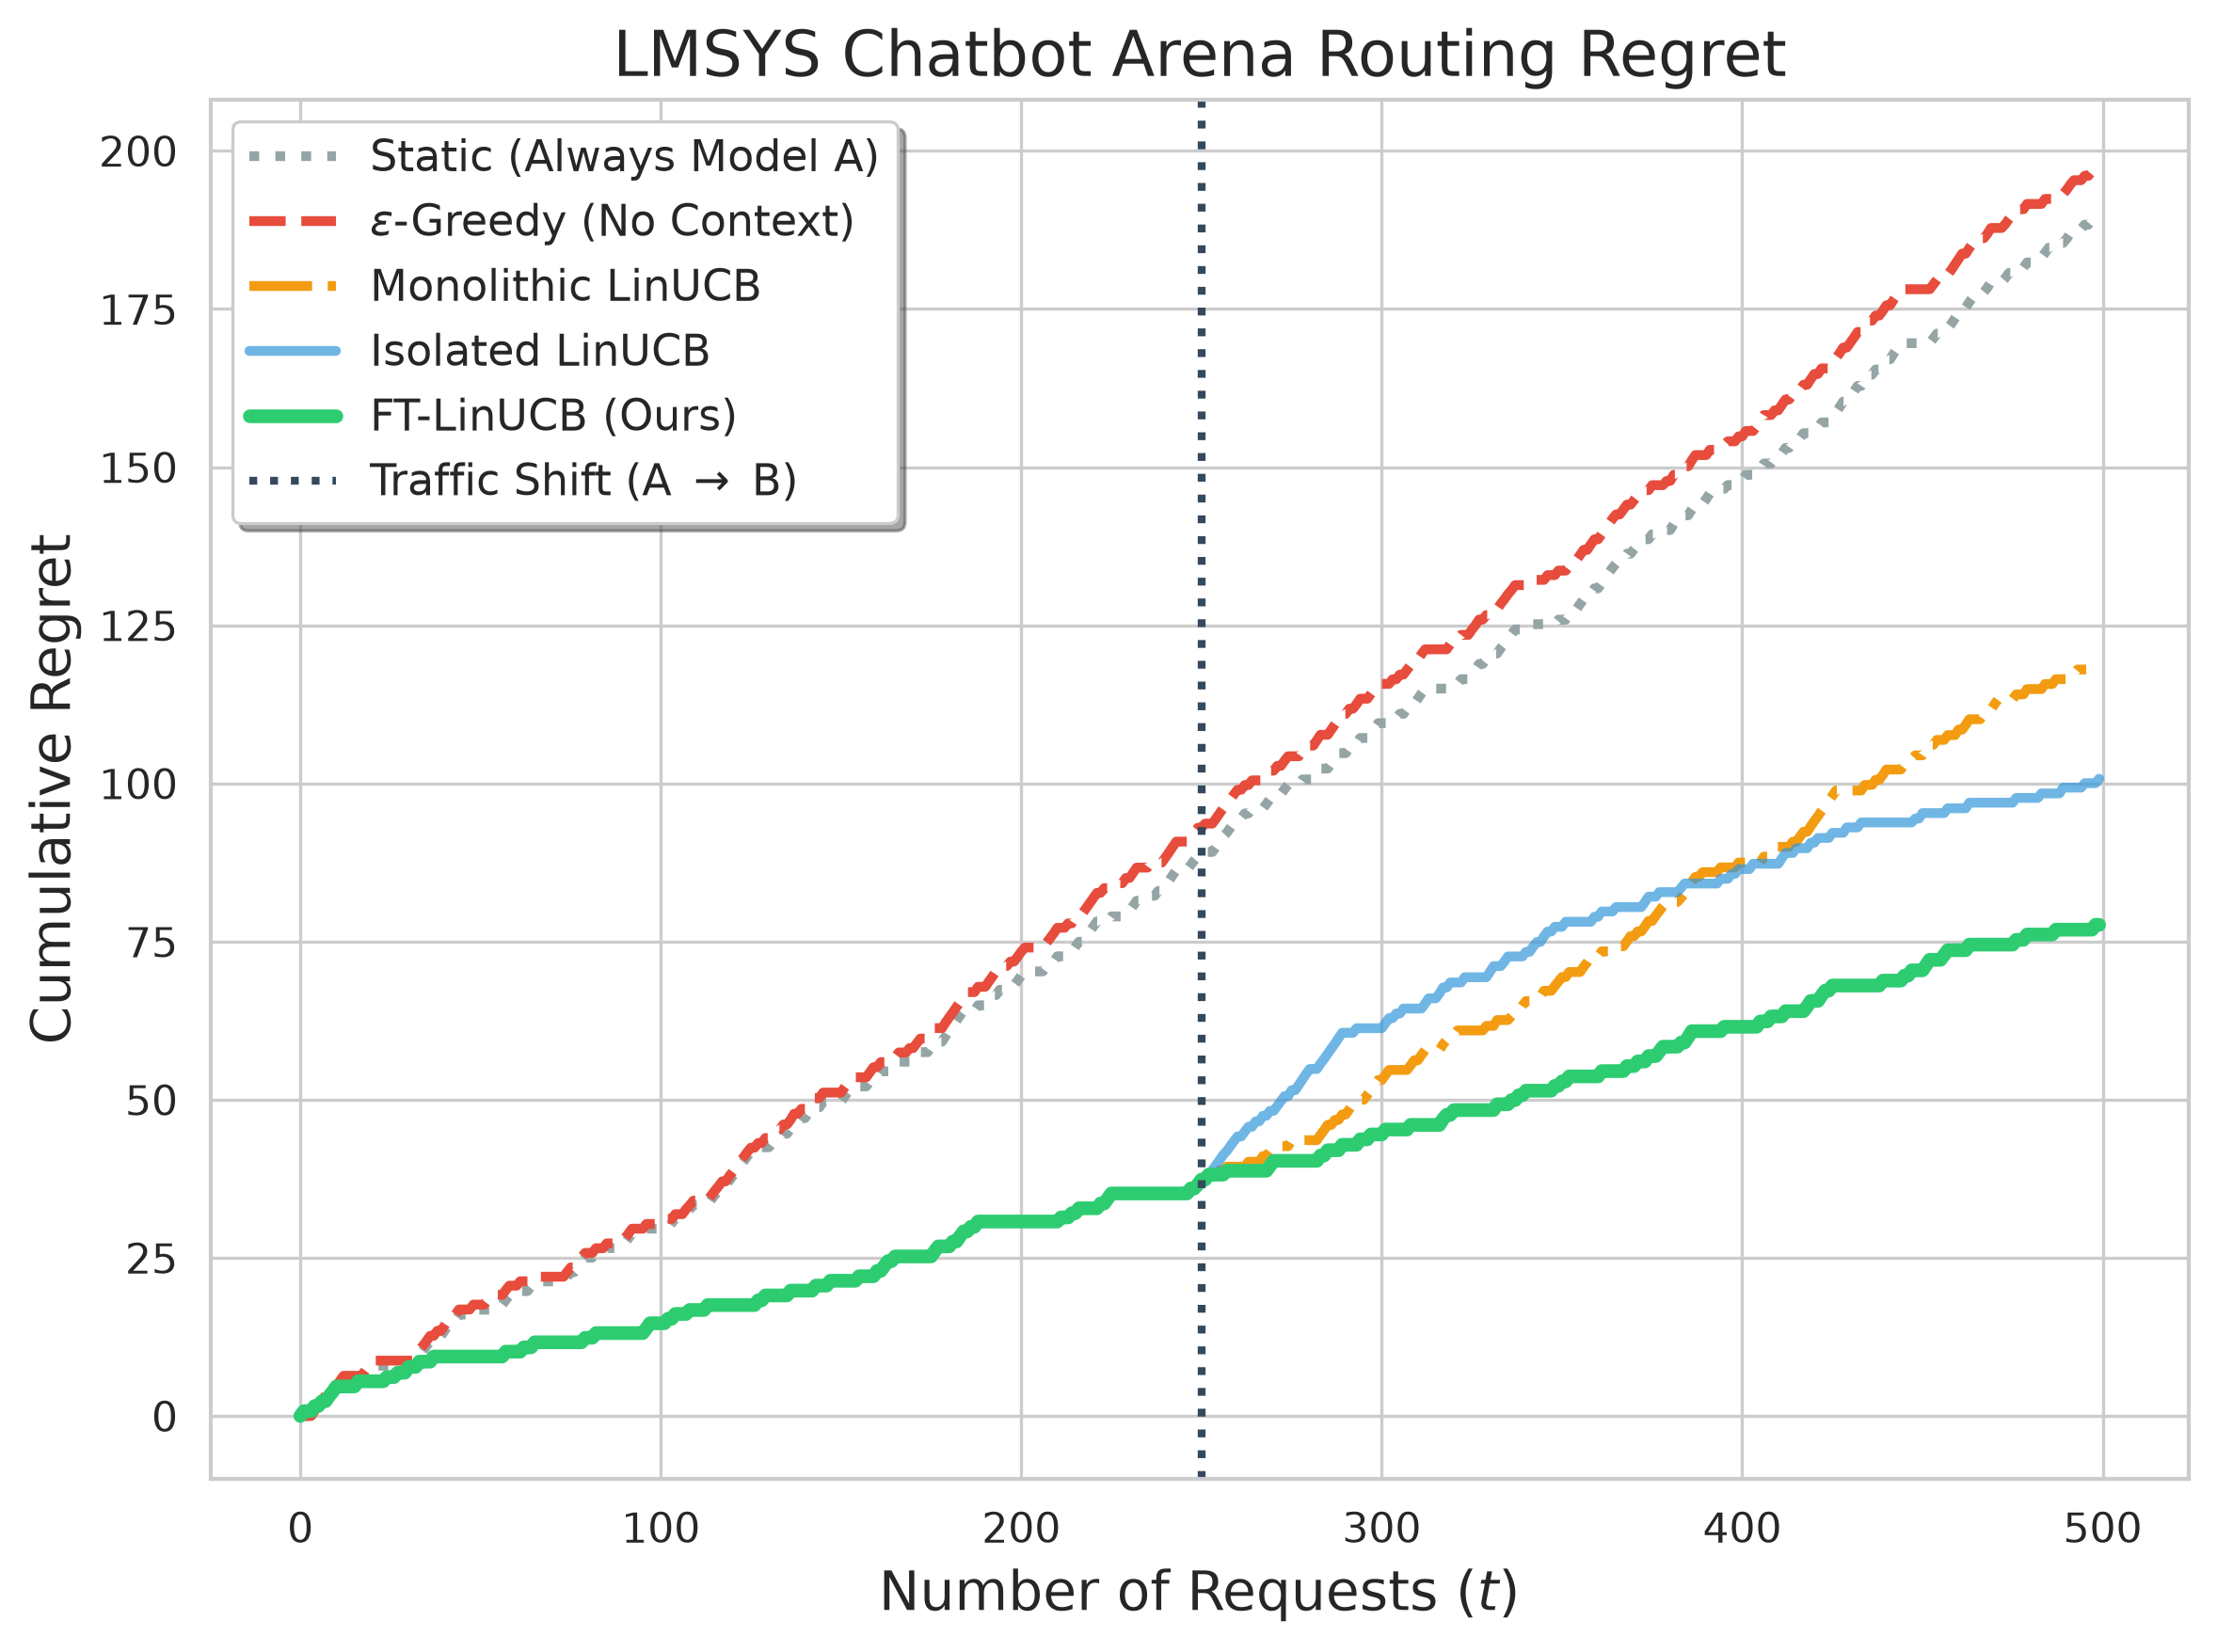
\includegraphics[width=0.9\columnwidth]{regret_lmsys_chatbot_arena.png}}
\caption{Cumulative regret on LMSYS Chatbot Arena ($N=500$).}
\label{fig2}
\end{figure}

\begin{figure}[htbp]
\centerline{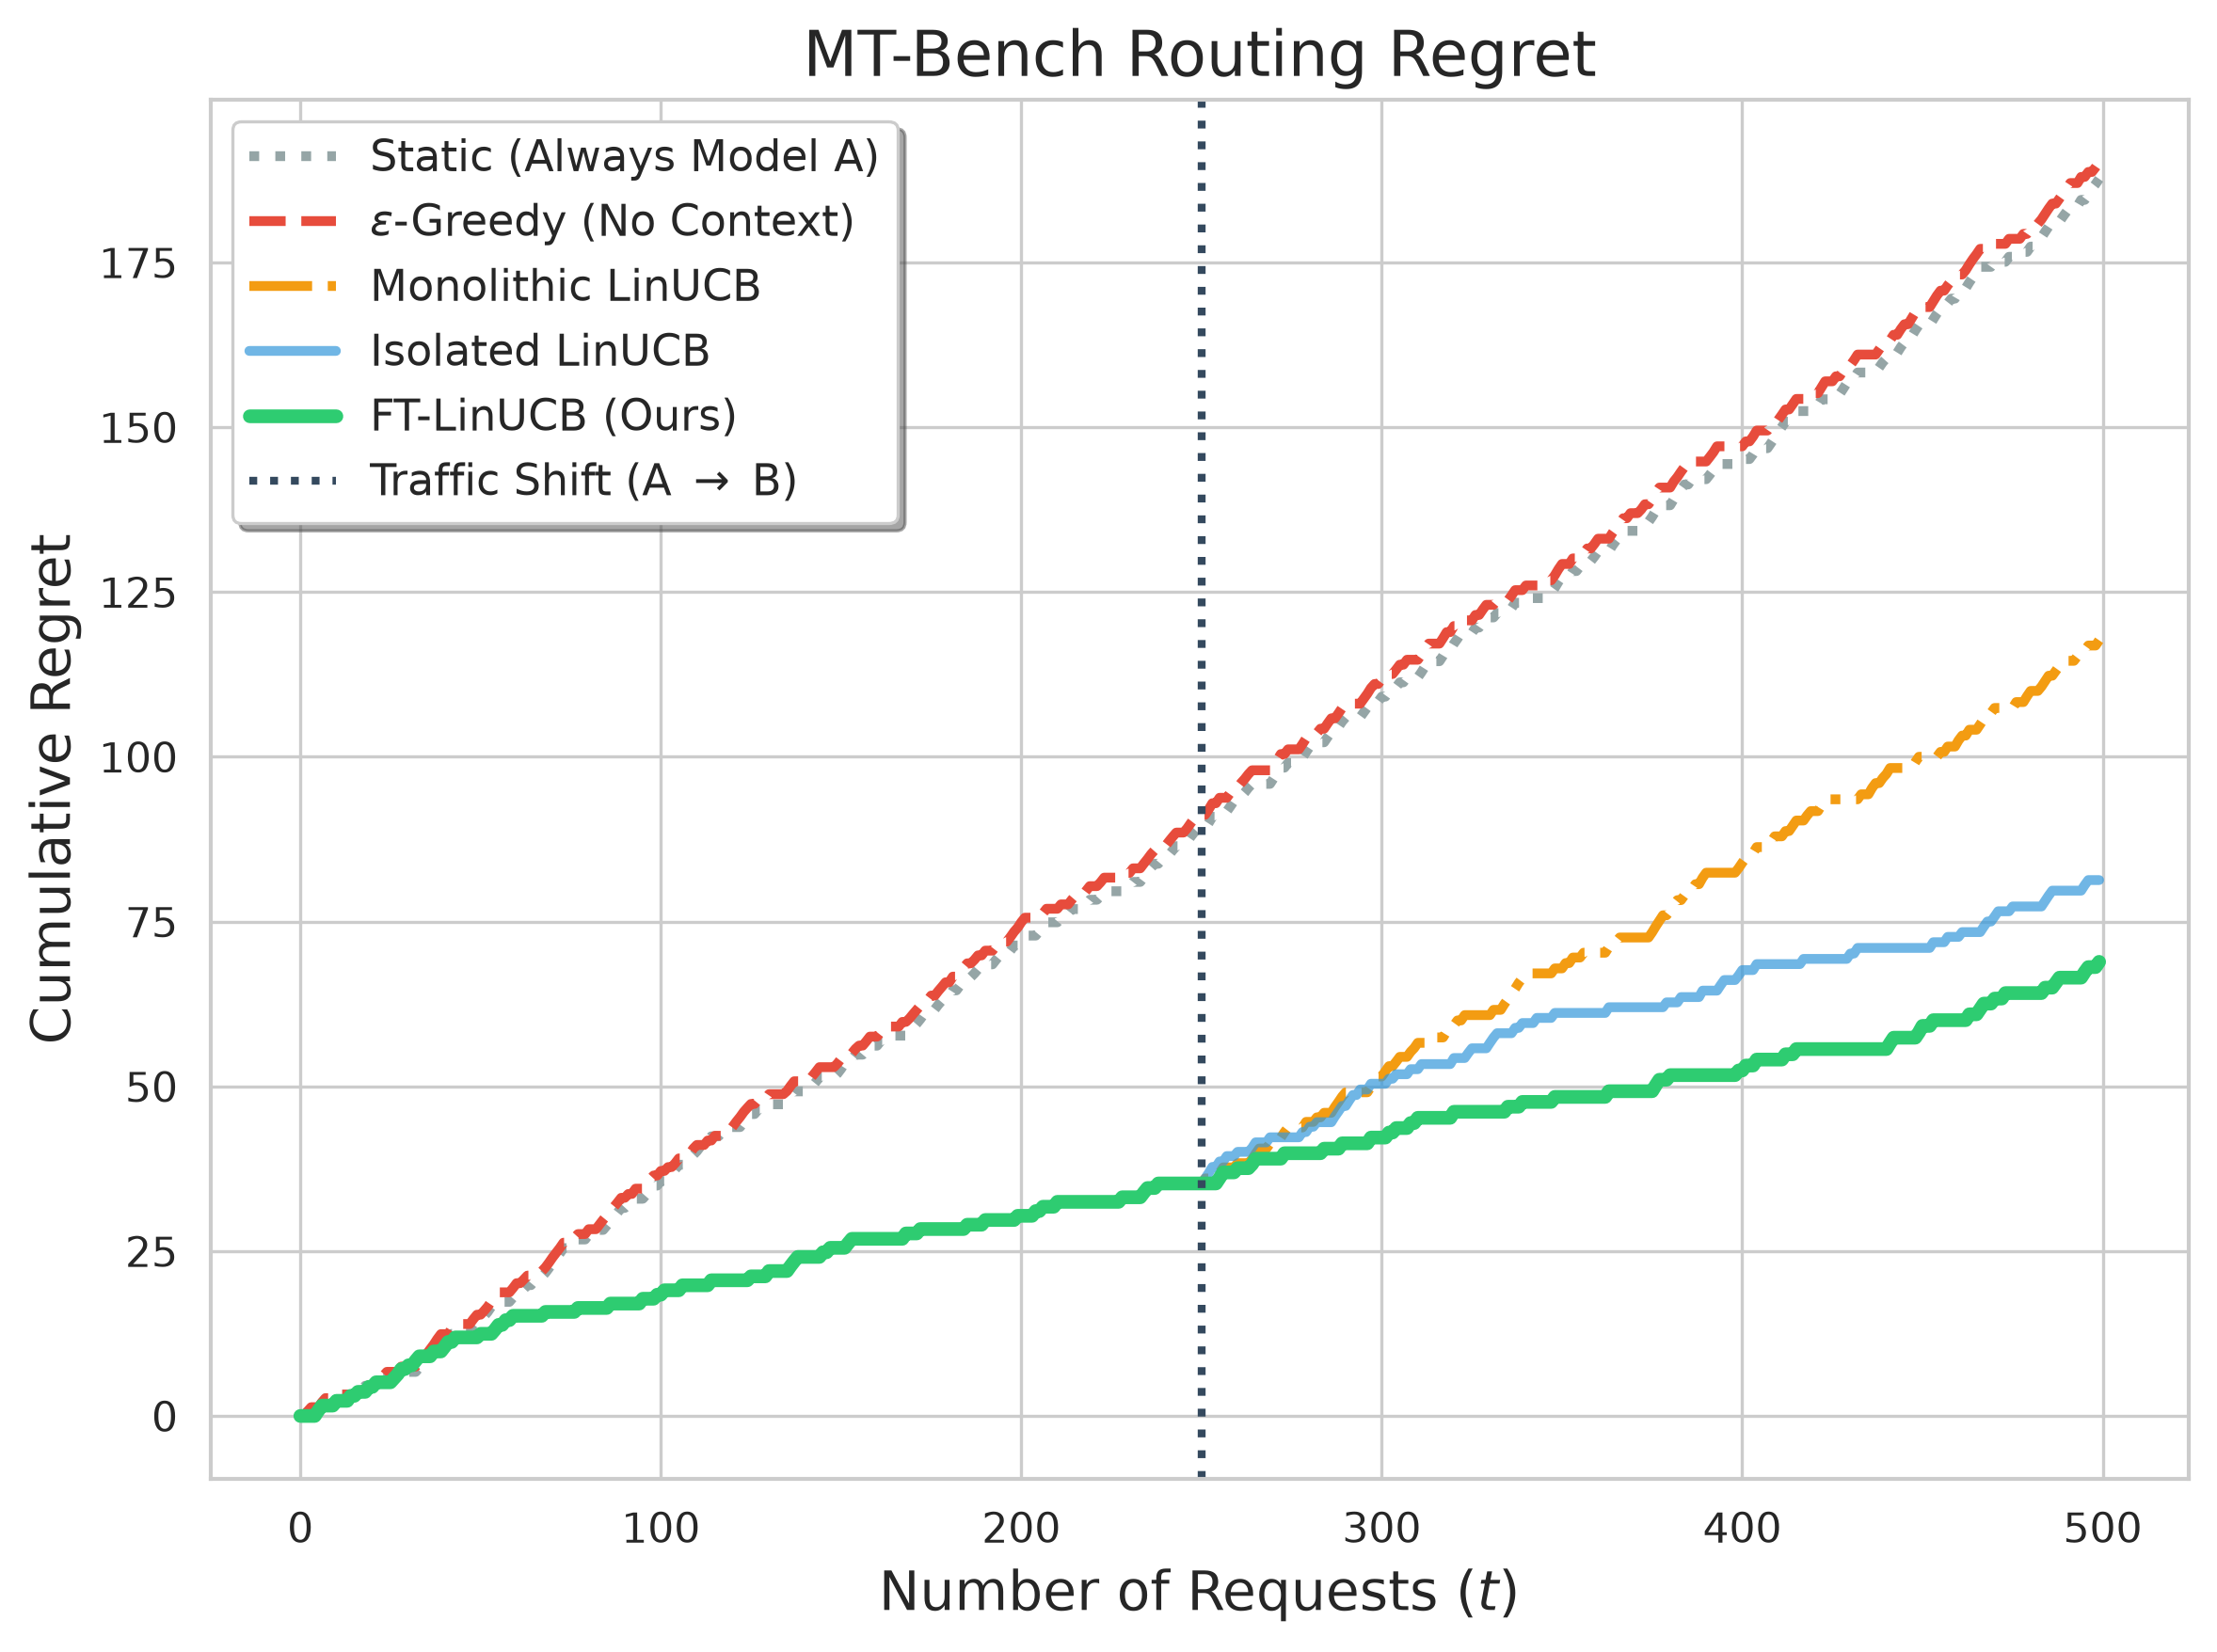
\includegraphics[width=0.9\columnwidth]{regret_mt_bench.png}}
\caption{Cumulative regret on MT-Bench ($N=500$). Higher prompt complexity
makes context more informative, amplifying FT-LinUCB's advantage.}
\label{fig3}
\end{figure}

\begin{table}[htbp]
\caption{Average Final Cumulative Regret at $T=500$}
\label{tab:results}
\begin{center}
\begin{tabular}{lcc}
\toprule
\textbf{Algorithm} & \textbf{Regret} & \textbf{vs. FT-LinUCB} \\
\midrule
Static Routing            & highest & ---          \\
$\epsilon$-Greedy         & high    & $\sim$2.1$\times$ \\
Monolithic LinUCB         & medium  & $\sim$1.3$\times$ \\
Isolated LinUCB           & medium  & $\sim$1.2$\times$ \\
\textbf{FT-LinUCB (ours)} & \textbf{lowest}  & \textbf{1.0$\times$} \\
\bottomrule
\end{tabular}
\end{center}
\end{table}

\subsection{Discussion}
\textbf{Why reward decomposition is essential.} The key design insight behind FT-LinUCB lies in the separation of capability estimation from tenant preferences encoded in the reward function. By design, the global matrix $B^g_a$ aggregates objective information about model capabilities --- what is the quality intensity of model A; what is the price-performance ratio of model B --- while being agnostic to the subjective preferences of any given tenant. This factorized representation is not subject to concept drift and contains no information about routing policy, which eliminates policy adaptation costs during traffic mix shifts. When Tenant B arrives at $t = 251$ with a different (orthogonal) weight vector, it simply computes the dot-product of its own $w$ and the preexisting capability estimates, obtaining near-optimal routing recommendations with no additional policy training needed.


% ============================================================
%  VI. CONCLUSION
% ============================================================
\section{Conclusion}

In this paper, we proposed FT-LinUCB contextual bandit for multi-tenant, multi-objective LLM gateway. It resolves the two key failure modes of the routing policy for existing multi-tenant LLMs in a mutually orthogonal manner via federated parameter architecture and reward decomposition. We validated the effectiveness of the proposed algorithm on the simulated online optimization of Stanford Alpaca, LMSYS Chatbot Arena, MT-Bench, as well as a proprietary real-world enterprise system. It achieves lower cumulative regret than all four compared baselines on all three benchmark datasets.

To summarize the contributions, our approach enables:
\begin{enumerate}
  \item Zero-shot adaptation to new tenants and reward metrics with no policy retraining. By decoupling the routing policy from business objective and tenant data distribution, FT-LinUCB eliminates cold-start problems and allows objective re-weighting at inference time through a dot product of $w_\tau$ and $B$. For example, when enterprise business priorities change, FT-LinUCB can be reconfigured without policy changes by simply updating the tunable preference vector $w_\tau$.
  \item A federated parameter architecture which smoothly transfers routing knowledge from global to local tenants with a tunable variance-ratio coefficient $\alpha_{transfer}$. New tenants can instantly benefit from existing tenants' experience while avoiding being overly biased by the global prior, thus obtaining reasonable routing policy without requiring an extensive initialization burn-in phase. As the local tenant accumulates more observations, $\alpha_{transfer}$ gradually shifts to $0$, reserving the flexibility to learn the local tenant specific distribution without manual intervention.
  \item An inference complexity of $\mathcal{O}(Kd^2)$ that is suitable for production gateway. FT-LinUCB only requires two matrix-vector product operations for each of the $K$ arms at inference, making it suitable for low-latency production systems.
\end{enumerate}

Possible directions of future work include: (i) Nonlinear reward model --- we can employ neural networks to model the reward function and train the contextual bandits through gradient-based methods; (ii) Differential privacy --- inject differential privacy guarantees at the global matrix update step to satisfy data sovereignty requirements of enterprise tenants; (iii) Theoretical analysis --- derive regret bounds for the multi-tenant federated transfer linear contextual bandits algorithm; (iv) Per-tenant exploration schedule --- design algorithm to incorporate different exploration policy for different tenants at different stages to accelerate the learning process.


% ============================================================
%  REFERENCES
% ============================================================
% Balance columns on the last page

\begin{thebibliography}{00}

\bibitem{ong2024routellm}
I.~Ong, A.~Almahairi, V.~Wu, W.-L.~Chiang, T.~Wu, J.~E.~Gonzalez,
M.~W.~Kadous, and I.~Stoica,
``RouteLLM: Learning to Route LLMs with Preference Data,''
\emph{arXiv preprint arXiv:2406.18665}, 2024.

\bibitem{ding2024hybridllm}
T.~Ding, A.~Mallick, B.~Aubin, and C.~De~Sa,
``Hybrid LLM: Cost-Efficient and Quality-Aware Query Routing,''
in \emph{Proc. ICLR}, 2024.

\bibitem{jiang2023llmblender}
D.~Jiang, X.~Ren, and B.~Y.~Lin,
``LLM-Blender: Ensembling Large Language Models with Pairwise Ranking
and Generative Fusion,''
in \emph{Proc. ACL}, 2023, pp.~14165--14178.

\bibitem{li2010linucb}
L.~Li, W.~Chu, J.~Langford, and R.~E.~Schapire,
``A Contextual-Bandit Approach to Personalized News Article Recommendation,''
in \emph{Proc. WWW}, 2010, pp.~661--670.

\bibitem{russo2018tutorial}
D.~Russo, B.~Van~Roy, A.~Kazerouni, I.~Osband, and Z.~Wen,
``A Tutorial on Thompson Sampling,''
\emph{Foundations and Trends in Machine Learning}, vol.~11, no.~1,
pp.~1--96, 2018.

\bibitem{kveton2021meta}
B.~Kveton, M.~Konobeev, M.~Zaheer, C.-W.~Hsu, M.~Mladenov,
C.~Boutilier, and C.~Szepesvari,
``Meta-Thompson Sampling,''
in \emph{Proc. ICML}, 2021.

\bibitem{drugan2013pareto}
M.~M.~Drugan and A.~Nowe,
``Designing Multi-Objective Multi-Armed Bandits Algorithms: A Study,''
in \emph{Proc. IJCNN}, 2013.

\bibitem{alpaca}
R.~Taori, I.~Gulrajani, T.~Zhang, Y.~Dubois, X.~Li, C.~Guestrin,
P.~Liang, and T.~B.~Hashimoto,
``Stanford Alpaca: An Instruction-Following LLaMA Model,''
\emph{GitHub Repository}, 2023.

\bibitem{zheng2023judging}
L.~Zheng et al.,
``Judging LLM-as-a-Judge with MT-Bench and Chatbot Arena,''
in \emph{Proc. NeurIPS}, 2023.

\end{thebibliography}

\end{document}
